\documentclass{article}
\usepackage[utf8]{inputenc}
\usepackage[T1]{fontenc}
\usepackage{graphicx}
\usepackage{amsmath}
\usepackage{wrapfig}
\usepackage[top=1in, bottom=1.25in, left=1.1in, right=1.1in]{geometry}

\title{Reporte - Actividad 9: wxMaxima}
\author{García Monge Itzel Alexia}
\date{18 de Abril, 2018}


\begin{document}
\maketitle
\section{wxMaxima}
Macsyma es una sistema de álgebra computacional que inició en los años sesenta del cual tiene su base Maxima. Un software de los años sesenta no tenía la intención de ser visual, sino de correr en una línea de comando de sólo texto. Por lo tanto, wxMaxima fue creado para tener esa imagen visual del mundo actual al tener las opciones de escribir texto, hacer reportes e incluir el menú de comandos.

\subsection{Escribir Texto Explicativo}
Para escribir texto o agregar un título, sección, subsección o subsubsección puedes intentar dos diferentes métodos. El primer método  es ir al menú y seleccionar \textbf{ celda, insertar texto$/$título$/$entrada}. En esta sección puedes agregar imágenes así como salto de página. Cada celda es interpretado como un párrafo, incluso si agregas salto entre líneas estas no serán interpretadas.

El segundo método es más práctico y rápido, pues consiste en usar el comando \textbf{ctrl} más un número:
\begin{itemize}
\item \textbf{ctrl + 1:} Empezar un nuevo cuadro de texto

\item \textbf{ctrl + 2:} Añadir título

\item \textbf{ctrl + 3:} Añadir sección.

\item \textbf{ctrl + 4:} Añadir subsección.

\item \textbf{ctrl + 5:}Añadir subsubsección.
\end{itemize}

También es posible usar comandos para guardar un proyecto:
\begin{itemize}
\item \textbf{ctrl + s:} Guardar

\item \textbf{ctrl + shift + s:} Guardar como
\end{itemize}



\section{Manual de Integración}

\subsection{Tipos de Integrales}

\begin{itemize}
\item\textbf{integrate}\textit{integrate (expr, x)} , \textit{integrate (expr, x, a, b)}\textbf{:} intenta calcular simbólicamente la integral de \textit{expr} con respecto a \textit{x}. Mientras que \textbf{integrate (expr,x)} es una integral indefinida, \textbf{integrate(expr, x, a, b)} es una integral definida con límites de integración \textit{a, b}. Es importante recordar que los límites no deben contener a x. En los límites de integración \textit{a} debe ser menor o igual a \textit{b}, en caso de ser iguales, la integral será igual a cero.


	\begin{center}
    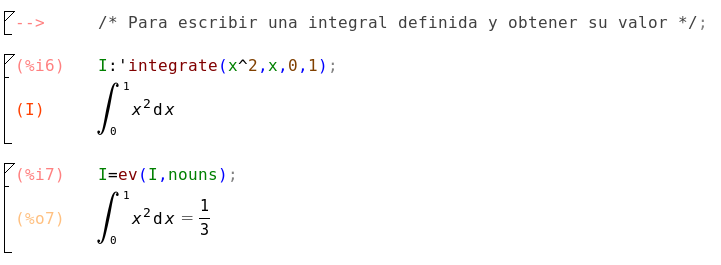
\includegraphics[height=4cm]{intdefinida.png}
    \end{center}

\item \textbf{dblint} \textit{(f, r, s, a, b)}\textbf{:} doble integral que usa el método de la regla de Simpson en las direcciones de $x$ y $y$ para calcular la integral, siendo \textit{s, r} escritas en función de una variable, mientras \textit{b, a} son puntos flotantes. Es requerido que las funciones \textit{f, r, s} sean compiladas antes de usa \textbf{dblint} ya que esto aumentará la velocidad de los cálculos.


\item\textbf{quad\_qags:} realiza la integración numérica, regresando un valor en lugar del valor simbólico utilizando funciones cuadráticas para aproximar la función y obtener una aproximación precisa a la integral. 

El resultado es regresado como una lista de cuatro elementos: el primero siendo el valor aproximado de la integral; el segundo el máximo error de estimación; el tercero es la información del número de funciones cuadráticas que fueron utilizadas para aproximar el valor; mientras que el cuarto da un código ERROR.

	\begin{center}
    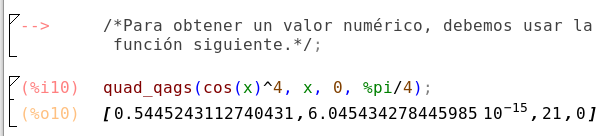
\includegraphics[height=2.5cm]{valornum.png}
    \end{center}

\item\textbf{defint}\textit{(expr, x, a, b)}\textbf{:} intenta calcular una integral definida, es llamada cuando los límites de la integración están especificados. En algunos casos es suficiente con usar el comando \textbf{integrate()}.


\item\textbf{integration\_constant , integration\_constant\_counter:} 
integration\_constant
Valor default: \%C. 

integration\_constant\_counter
Valor default: 0

Cuando una constante de integración es introducida por una integral indefinida de una ecuación, el nombre de esa constante es construida al concatenar \textbf{integration\_constant} y \textbf{integration
\_constant\_counter}.

A \textbf{integration\_constant} puede asignarsele cualquier símbolo, mientras que \textbf{integration
\_constant\_counter} es incrementado antes de construir la siguiente constante de integración.


	\begin{center}
    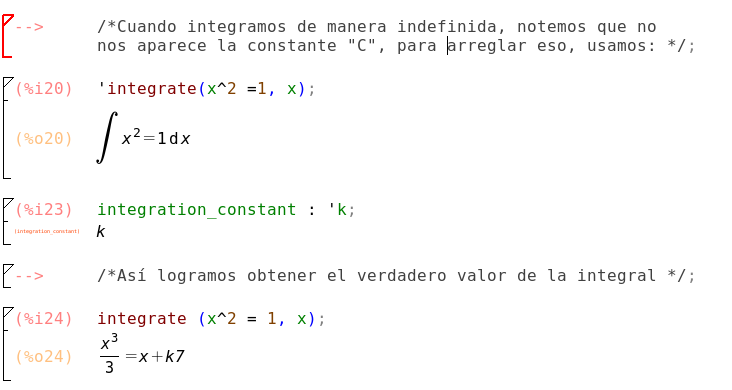
\includegraphics[height=6cm]{constantek.png}
    \end{center}

\item \textbf{ldefint}\textit{(expr, x, a, b)}\textbf{:} intenta calcular la integral definida de \textit{expr}  usando límites para evaluar la integral indefinida de \textit{expr} con respecto a \textit{x}, usando a \textit{b} como límite superior y \textit{a} como inferior. Si no logra calcularse, \textbf{ldefint} regresa una expresión conteniendo los límites en forma noun. \textbf{ldefint} no es llamada desde \textbf{integrate()}, así que esta función puede no reconocer algunos casos especiales.

\end{itemize}




\subsection{Variables de Integración}

\begin{itemize}
\item \textbf{changevar} \textit{expr, f(x,y), y, x}\textbf{:} hace cambios de variable dados por $f(x,y) = 0$ en todas las integrales ocurriendo en \textit{expr} con integración respecto a $x$, convirtiéndose $y$ en la nueva variable. 

	\begin{center}
    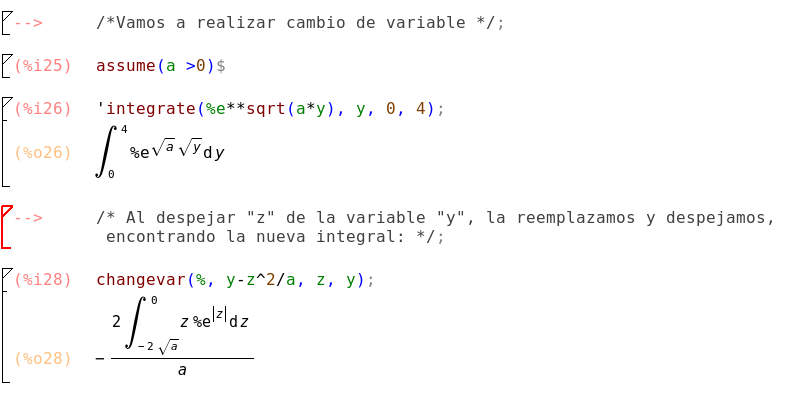
\includegraphics[height=6cm]{cambiodevar.png}
    \end{center}


\item \textbf{ilt}\textit{(expr, s, t)}\textbf{:} calcula la transformación de Laplace de \textit{expr}, el cual debe ser la proporción de polinomios cuyo denominador tenga factores lineales y cuadráticos, con respecto a \textit{s} y el parámetro \textit{t}. 

Usando \textbf{ilt} y la función \textbf{laplace} con funciones \textbf{solve} podemos resolver ecuaciones diferenciales integrables.

	\begin{center}
    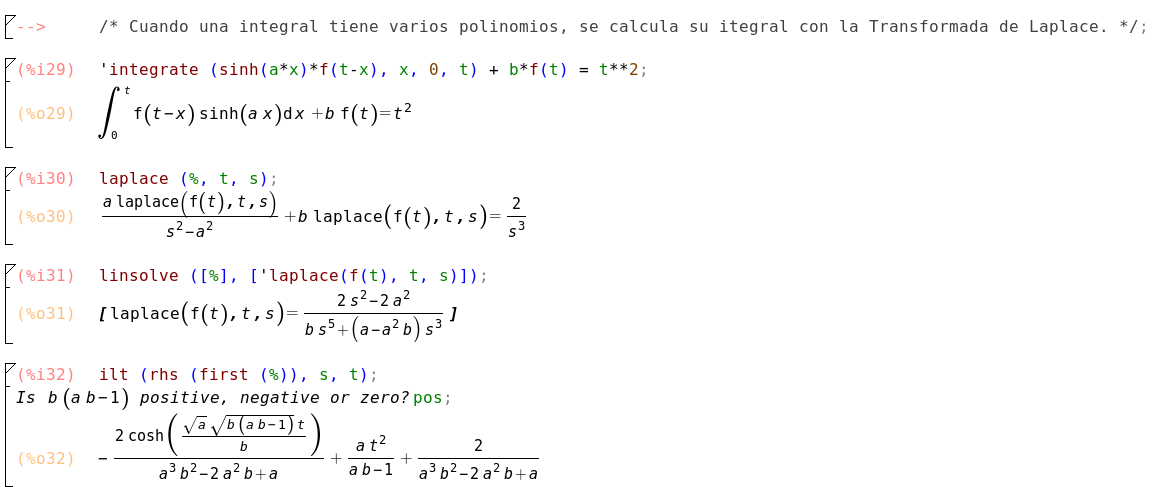
\includegraphics[height=7cm]{Laplace.png}
    \end{center}

\item \textbf{intanalysis:} su valor default es TRUE, haciendo que la integral definida trate de encontrar polos en el integrando en el intervalo de integración. Si las hay, entonces la integral es evaluada como una integral de valor principal. De lo contrario, no se asume que existan polos.


\item \textbf{integrate\_use\_rootsof:} su valor default es FLASO, haciendo que el integrando regrese una integral sin resolver de una función racional en forma \textit{noun}. 

En el caso contrario, el denominador de la funcional racional no puede factorizarse, así que el integrando regresa una integral en una forma donde la suma de sus raíces sea del denominador.

	\begin{center}
    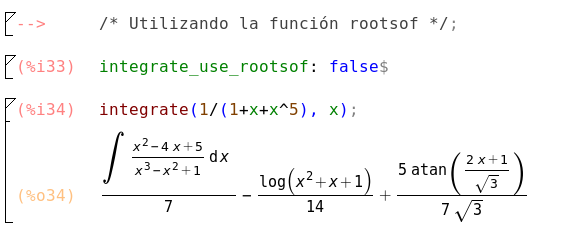
\includegraphics[height=4cm]{rootsof.png}
    \end{center}

\item\textbf{residue}\textit{(expr, z, z\_0)}\textbf{:} calcula el residuo en el plano complejo de la expresión \textit{expr} cuando la variable $z$ asume el valor z\_0. El residuo es el coeficiente de (z - z\_0)\^(-1) en la serie de Laurent para \textit{expr}.


\item\textbf{risch}\textit{(expr, x)}\textbf{:} integra \textit{expr} con respecto a \textit{x} usando el algoritmo de Risch. Esta función se encarga de exponentes y logaritmos anidados, siendo estos la parte principar que el integrando no puede hacer.

	\begin{center}
    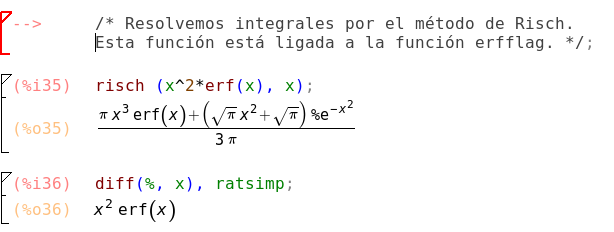
\includegraphics[height=4cm]{risch.png}
    \end{center}

\item \textbf{erfflag:} su valor default es TRUE, en caso contrario, detiene a la función \textbf{risch} de introducir la función \textbf{erf} en la respuesta-si hubiera un integrando en primer lugar.
\end{itemize}




\section{Problema}
A continuación se ilustrará un problema utilizado en el curso de \textit{Cálculo IV}, en donde se desea obtener la longitud de un cardioide. 

	\begin{center}
    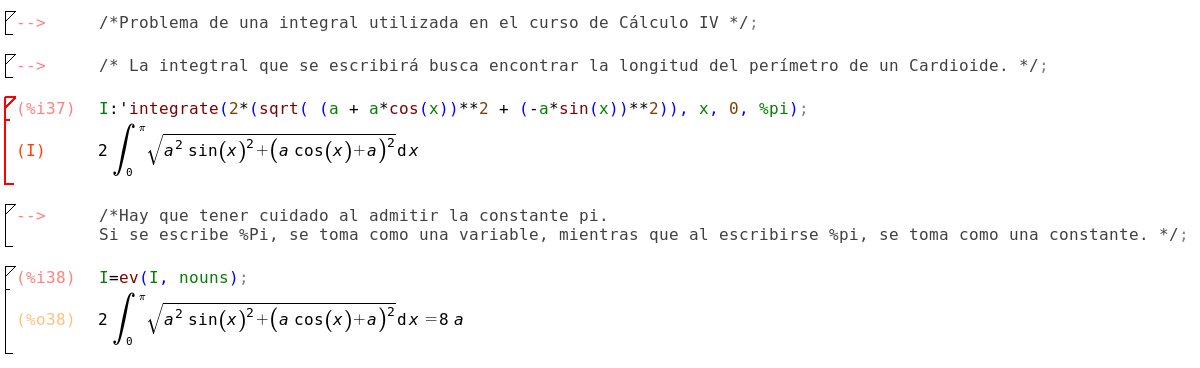
\includegraphics[height=5cm]{Problema.png}
    \end{center}

Además, se graficó en \textit{wxMaxima} la figura para una visualización más fácil del problema, el cual incluiremos a continuación.

	\begin{center}
    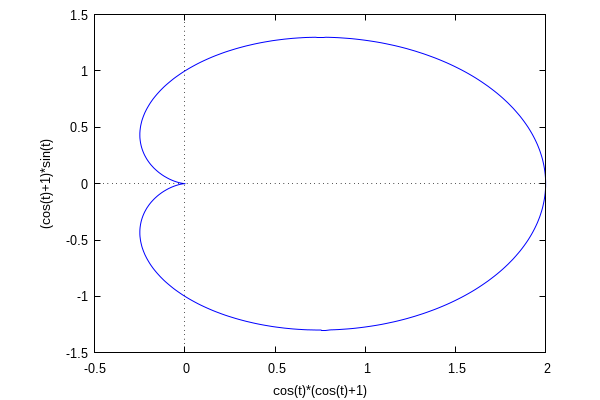
\includegraphics[height=7cm]{cardioide.png}
    \end{center}

\section{Apéndice}
\begin{enumerate}
\item \textbf{¿Cuál fue tu primera impresión de wxmaxima?} Me gustó lo poco que trabajé con ella en el transcurso de está actividad, me sentí más cómoda programando con ella a comparación de $Pyhton$.

\item\textbf{¿Crees que esta herramienta puede ser útil en otros de tus cursos?} Absolutamente, es una herramienta que puede ser utilizada en la mayoría de mis cursos de primeros semestres, así como unos cuantos en los que me encuentro, como Cálculo II, III, IV y Álgebra Lineal I.


\item\textbf{¿Qué se te dificultó más en esta actividad?} Entender cómo funciona su lectura de código, qué interpreta como variable, cómo crear los comentarios, fue más que nada una dificultas presentada siempre que te enfrentas a un nuevo lenguaje de programación.

\item\textbf{¿Se te hizo compleja esta actividad? ¿Cómo la mejorarías?} Me pareció una muy buena actividad para introducirnos a un nuevo lenguaje de programación, aunque sea álgebra computacional. No le mejoraría nada.
\end{enumerate}


\section{Bibliografía}
\begin{itemize}
\item Maxima 5.41.0 Manual. Consultado: April 28, 2018

$http://maxima.sourceforge.net/docs/manual/maxima_singlepage.html\#SEC98$

\item Maxima Tutorial. (2018). J.A. Villate. Consultado: April 28, 2018

$https://def.fe.up.pt/dynamics/maxima_tutorial.html$

\item Scot Childress. (2016). Integration. Consultado: April 28, 2018

$http://www.scotchildress.com/wxmaxima/$

\end{itemize}


\end{document}
